%% Requires compilation with XeLaTeX or LuaLaTeX
\documentclass[10pt,xcolor={table,dvipsnames},t]{beamer}

\usepackage[utf8]{inputenc}
\usepackage[spanish]{babel}
\usepackage{amssymb}
\usepackage{amsfonts,amsmath,amsthm} % Math packages
\usepackage{mathabx}
\usepackage{mathtools}
\usepackage{tikz}
\usepackage{paralist}
\usepackage{xypic}
\usepackage{graphicx}
\graphicspath{ {./images/} }
\usepackage[lofdepth,lotdepth]{subfig}
\usepackage{float}
\usepackage{enumitem}
\usetikzlibrary{babel,automata,positioning,arrows}
\newcommand{\Tau}{\mathrm{T}}
\newtheorem{ejemplo}{Ejemplo}
\definecolor{com}{RGB}{236, 93, 87}
\definecolor{proc}{RGB}{125, 197, 82}
\definecolor{muller}{RGB}{81, 167, 249}
\definecolor{map}{RGB}{179, 106, 226}
\definecolor{prov}{RGB}{243, 144, 25}
\definecolor{req}{RGB}{220, 189, 35}

\title{Auómatas para la vinculación parcial de servicios}
\author{Ezequiel Davidovich Caballero}
\institute{Departamento de Computación, Facultad de Ciencias Exactas y Naturales}
\date{11 de Noviembre 2020}


\begin{document}


\begin{frame}
\vspace{-2cm}
\begin{center}
\begin{tabular}{l}

\includegraphics[width=2cm]{logofcen.pdf}
\end{tabular}    
\end{center}

  \titlepage
  
  

{Director: Carlos G. Lopez Pombo}

\vspace{.2cm}

{Codirector: Ignacio Vissani}

\vspace{.2cm}

Buenos Aires, 2020

\end{frame}

% Uncomment these lines for an automatically generated outline.
%\begin{frame}{Outline}
%  \tableofcontents
%\end{frame}

\section{Introduction}
\begin{frame}{Intro (Motivación)}

\begin{center}
``Computing is becoming a utility and software a service. […] applications will no longer bea big chunk of software that runs on a computer but a combination of web services; and the platform for which developers write their programs will no longer be the operating system, but application servers.”
\end{center}
The Economist, May 2003
\begin{center}
“La computación se está volviendo una utilidad y el software un servicio. […] las aplicaciones van a dejar de ser un gran bloque de software que corre en una computadora para ser una combinación de servicios web; y la plataforma para la que los desarrolladores escriben sus programas dejará de ser un sistema operativo para ser servidores de aplicaciones.”    
\end{center}
The Economist, Mayo 2003
\end{frame}

\begin{frame}{API Economy}
\vspace{\fill}
 \textbf{Tools and Methods for Software Development section of H2020 work programme 14/15}\footnote{HORIZON 2020 – WORK PROGRAMME 2014 2015 LEIT – ICT. \url{https://ec.europa.eu/research/participants/data/ref/h2020/wp/2014_2015/main/h2020-wp1415-leit-ict_en.pdf}. pp. 23.}: 
 The quality levels required for complex and critical systems for example in terms of reliability, resilience and automatic adaptation, still represent a major challenge given current software development methods and tools. Breakthroughs in this area could significantly improve the growth and competitiveness of the European industry and encourage faster innovation cycles.
 
\vspace{\fill}

\textbf{Cloud Computing section of H2020 work programme 16/17}\footnote{HORIZON 2020 – WORK PROGRAMME20162017 LEIT – ICT. \url{https://ec.europa.eu/research/participants/data/ref/h2020/wp/2016_2017/main/h2020-wp1617-leit-ict_en.pdf}. pp. 19.} : Recent trends in cloud computing go towards the development of new paradigms (heterogeneous, federated, distributed clouds) as opposed to the current centralised model, with tight interactions between the computing and networking infrastructures.
\vspace{\fill}
\end{frame}

\begin{frame}{Service-oriented Computing}
% Service-oriented computing (SOC) es el paradigma de cómputo que utiliza servicios como elementos fundamentales para el desarrollo de aplicaciones. Para construir este modelo de servicios, SOC se basa en un modo de reorganizar el aplicaciones de software e infraestructura en un conjunto de servicios que interactúan entre sí.

En Service-oriented computing los sistemas de software tienen tres características distintivas:
\begin{itemize}
  \item \textbf{Reconfiguración dinámica:} la estructura del sistema varía en tiempo de ejecución a medida que este va requiriendo servicios externos para completar una tarea necesaria para cumplir su objetivo

  \item \textbf{Heterogeneidad intrínseca:} los servicios que se utilizan durante la ejecución se toman de repositorios y su naturaleza es desconocida fuera del contrato sobre el cual se establece el Service Level Agreement
  
  \item \textbf{Altamente no determinísticos:} los repositorios cambian a lo largo del tiempo como consecuencia de servicios que se registran y desregistran constantemente. Por lo tanto no hay garantía de que un mismo servicio satisfaga dos requerimientos idénticos 

\end{itemize}

\end{frame}

\section{ARN}

\begin{frame}{Asynchronous Relational Nets}
\begin{center}
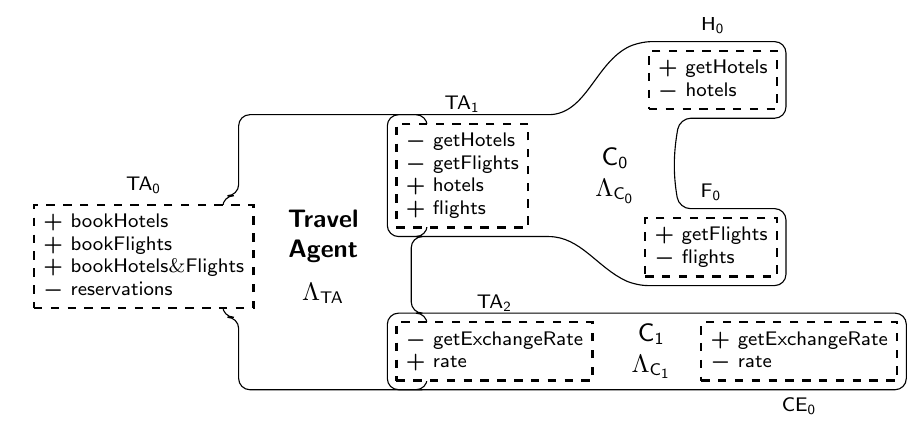
\includegraphics[scale=0.5]{images/ARN0.png}
\end{center}
\end{frame}

\begin{frame}{Asynchronous Relational Nets \cite{fiadeiro:fase2011}}
\begin{center}
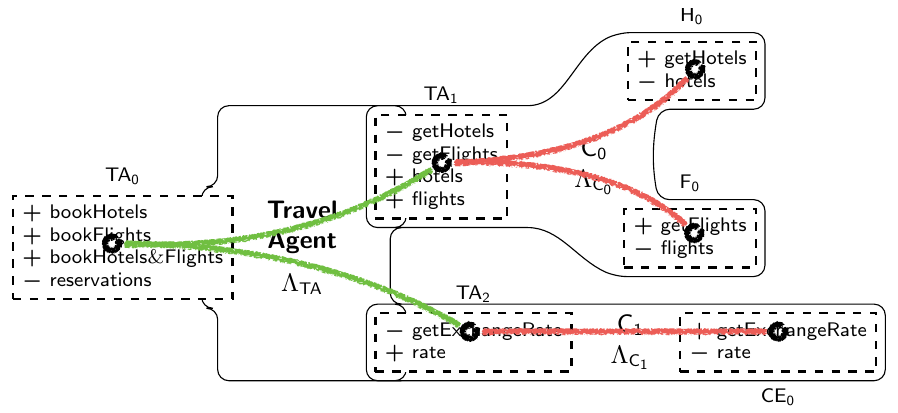
\includegraphics[scale=0.5]{images/ARN1.png}
\end{center}
Una ARN es una estructura bipartita basada en hipergrafos cuyos nodos son considerados \textbf{puertos}, y tiene dos tipos de hiperarcos, que se interpretan como \textcolor{com}{canales de comunicación} y \textcolor{proc}{pocesos}, respectivamente.
\end{frame}

\begin{frame}{Asynchronous Relational Nets \cite{fiadeiro:fase2011}}
\begin{center}
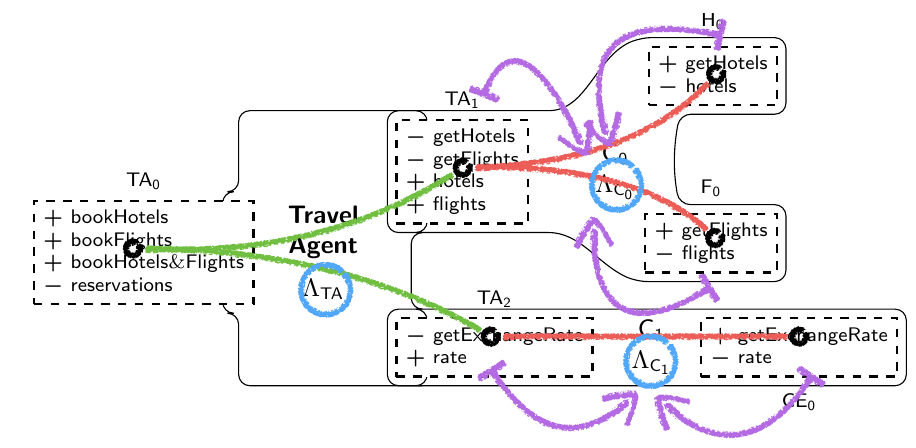
\includegraphics[scale=0.5]{images/ARN2.png}
\end{center}
Cada hiperarco es etiquetado con un \textcolor{muller}{autómata de Muller}. En el caso de los \textcolor{proc}{procesos} sobre el alfabeto de los \textbf{puertos} adyacentes y en el caso de los \textcolor{com}{canales de comunicación}, sobre un nuevo alfabeto al que los hiper ejes de los puertos se \textcolor{map}{mapean inyectivamente}  
\end{frame}

\begin{frame}{Asynchronous Relational Nets \cite{fiadeiro:fase2011}}
\begin{center}
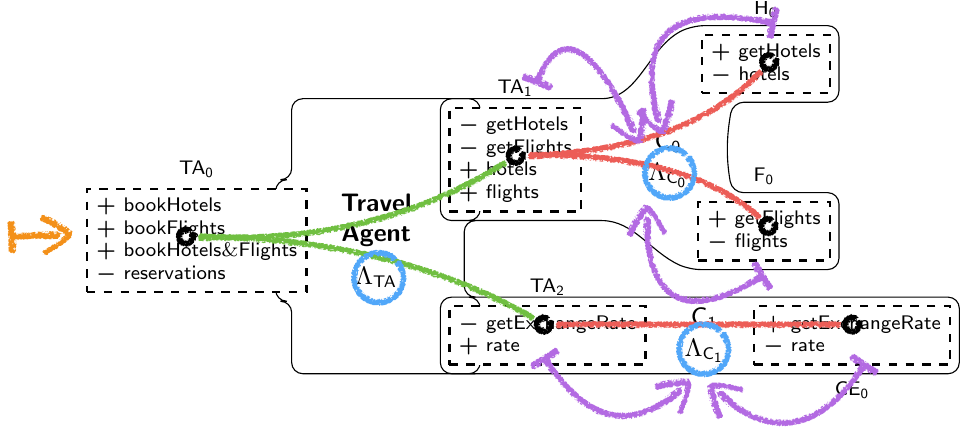
\includegraphics[scale=0.5]{images/ARN3.png}
\end{center}
Los nodos que son únicamente adyacentes a \textcolor{proc}{procesos} se denominan \textcolor{prov}{provides points}  
\end{frame}

\begin{frame}{Asynchronous Relational Nets \cite{fiadeiro:fase2011}}
\begin{center}
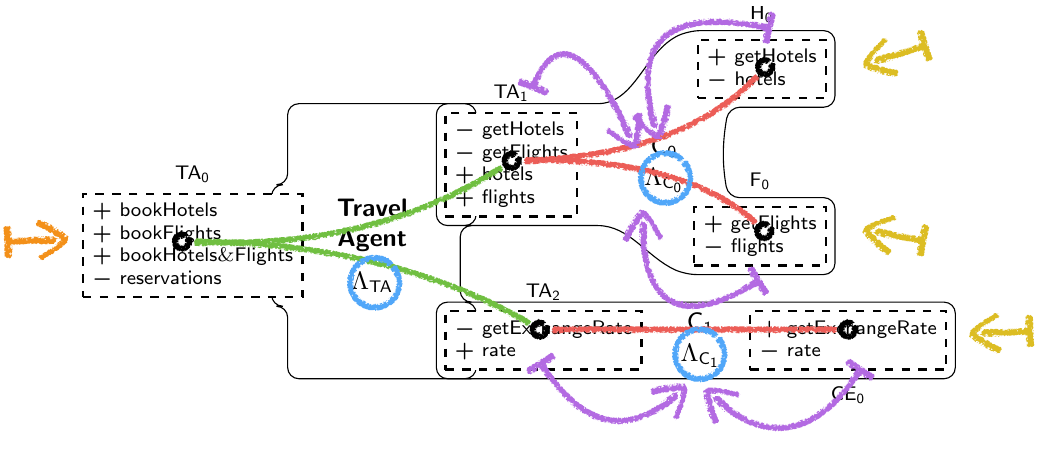
\includegraphics[scale=0.5]{images/ARN4.png}
\end{center}
Los nodos que son únicamente adyacentes a \textcolor{proc}{procesos} se denominan \textcolor{prov}{provides points}, mientras que aquellos adyacentes a \textcolor{com}{canales de comunicación} se denominan \textcolor{req}{requires points}  
\end{frame}

\begin{frame}{Asynchronous Relational Nets \cite{fiadeiro:fase2011}}
\begin{center}
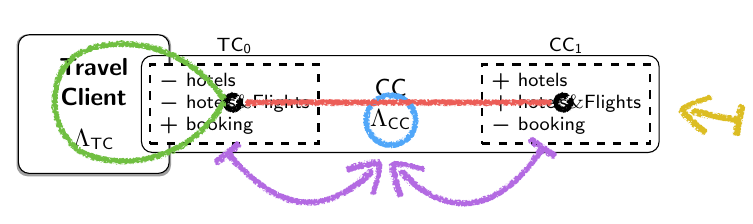
\includegraphics[scale=0.5]{images/ARN5.png}
\end{center}
Si una ARN tiene \textcolor{prov}{provides points}, se dice que es un \textbf{servicio} porque puede ser vinculado a través de los mismos.
\end{frame}

\begin{frame}{Asynchronous Relational Nets \cite{fiadeiro:fase2011}}
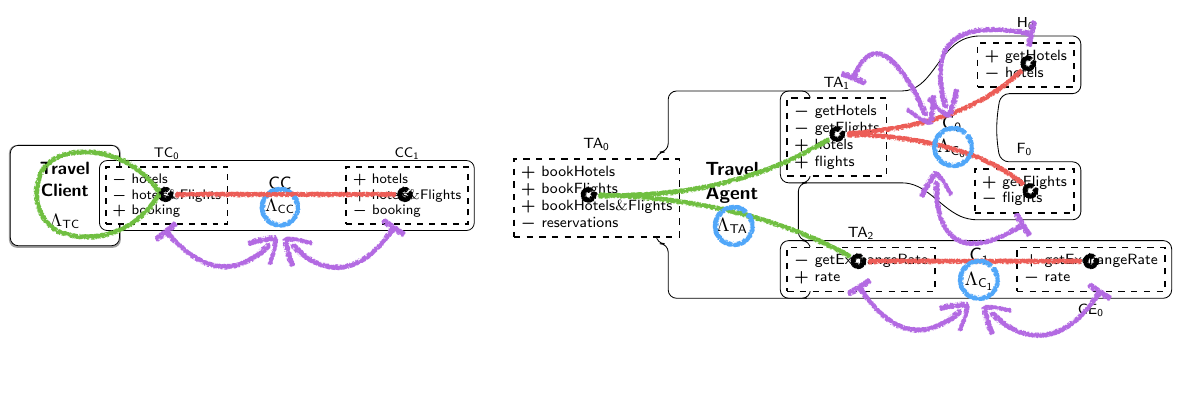
\includegraphics[scale=0.45]{images/ARN6.png}
\end{frame}


\begin{frame}{Asynchronous Relational Nets \cite{fiadeiro:fase2011}}
\begin{center}
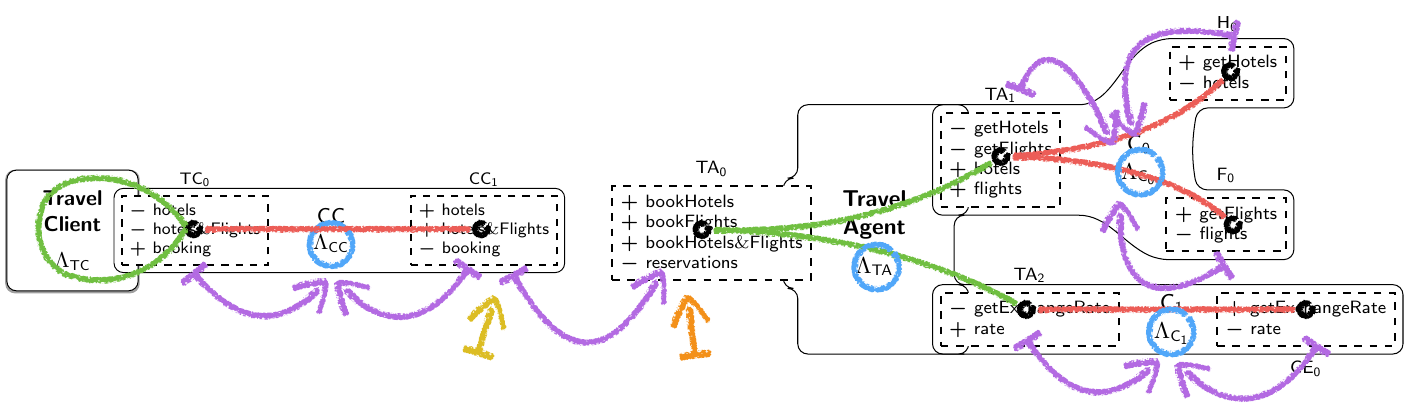
\includegraphics[scale=0.39]{images/ARN7.png}
\end{center}
La composición de una \textbf{actividad} con un \textbf{servicio} se realiza a través de un \textcolor{map}{mapeo inyectivo} del lenguaje de un \textcolor{req}{requires points} de una \textbf{actividad} al lenguaje de un \textcolor{prov}{provides points} de un \textbf{servicio}
\end{frame}

\begin{frame}{Asynchronous Relational Nets \cite{fiadeiro:fase2011}}
\begin{center}
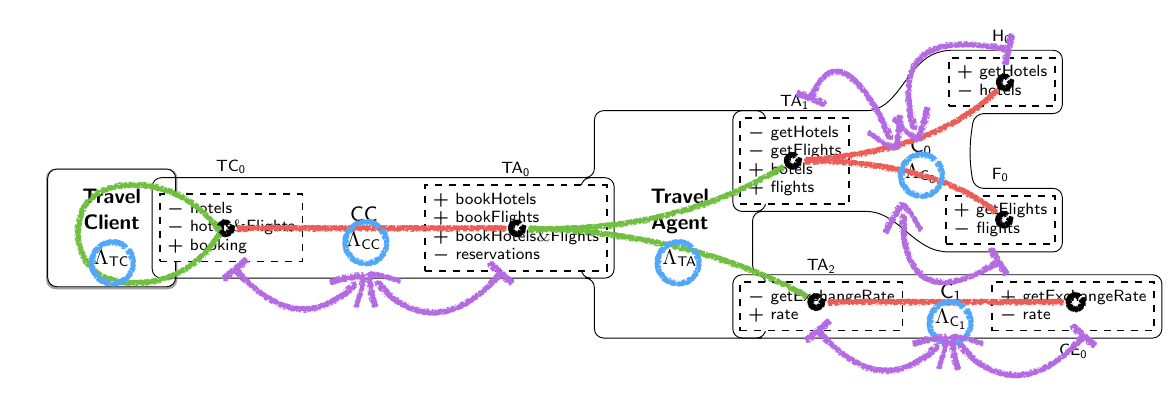
\includegraphics[scale=0.39]{images/ARN8.png}
\end{center}
La composición de una \textbf{actividad} con un \textbf{servicio} se realiza a través de un \textcolor{map}{mapeo inyectivo} del lenguaje de un \textcolor{req}{requires points} de una \textbf{actividad} al lenguaje de un \textcolor{prov}{provides points} de un \textbf{servicio}
\end{frame}


\begin{frame}{Asynchronous Relational Networks}
   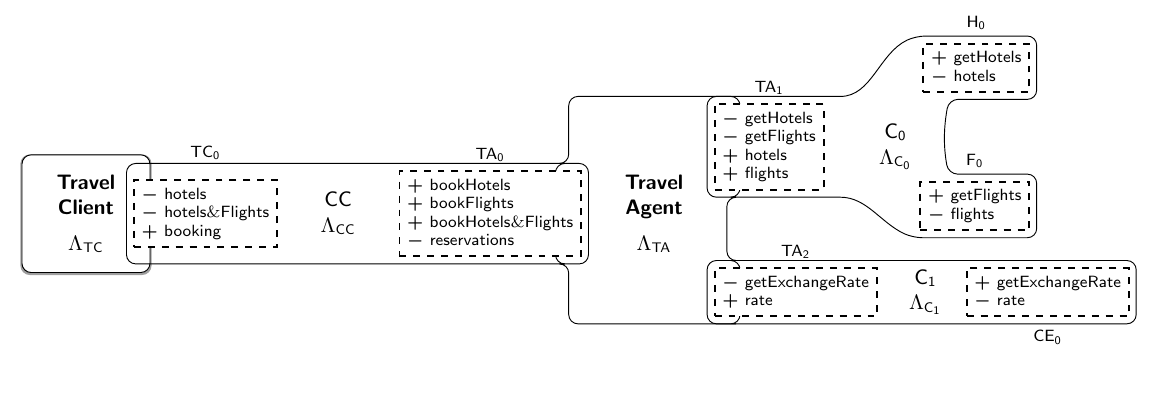
\includegraphics[scale=0.45]{images/ARN9.png}
Problema: el rol que tienen los autómatas de Muller que etiquetan los hiperarcos de comunicación es el de \textbf{orquestar} las interacciones entre procesos, obligando a los procesos a sincronizar sobre el al lenguaje compartido y posibilitando la asincronía sólo sobre las acciones internas.
\end{frame}

\begin{frame}{Communicating Relational Networks\cite{vissani:places15}}
\begin{center}
    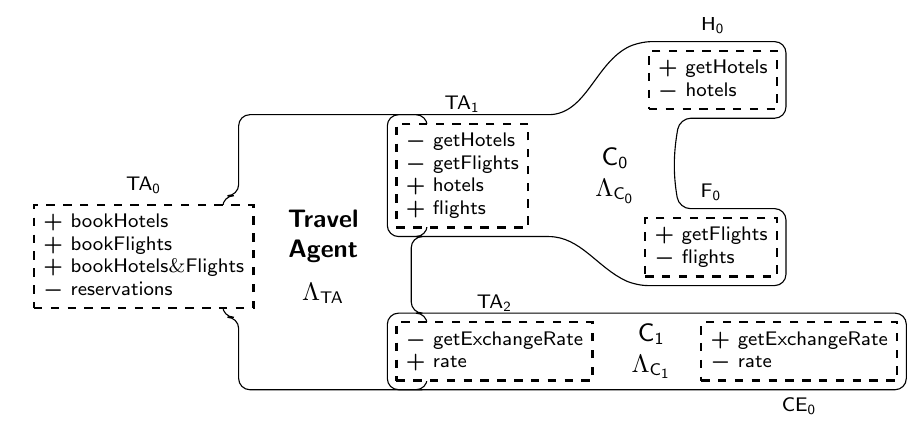
\includegraphics[scale=0.5]{images/ARN0.png}
\end{center}
Respuesta: Reemplazar los autómatas de Muller de los hiperarcos de comunicación por una descripción de una \textbf{coreografía} basada en intercambio de mensajes.
\end{frame}


\begin{frame}{Communicating Relational Networks}
\begin{itemize}
    \item \textbf{Coreografía (visión local) \cite{brand:jacm-30_2}:} las Communicating Finite State Machines (CFSMs)  son autómatas finitos cuyos ejes se etiquetan con:  \begin{inparaenum}[a.]\item $P!m$ indicando que se le envía el mensaje $m$ al participante $P$ o \item $P?m$ indicando que el participante $P$ recibe el mensaje $m$
     \end{inparaenum}
    \item \textbf{Coreografía (visión global) \cite{denielou:esop12}}: los global graphs son autómatas finitos cuyos ejes se etiquetan con $P \rightarrow Q:m$ indicando que el participante $P$ envía el mensaje $m$ a $Q$.
\end{itemize}
\end{frame}


\begin{frame}{Communicating Relational Networks}
\begin{itemize}
    \item \textbf{Provides point} (los puntos conectados sólo a hiperarcos de proceso): se etiquetan con una \textbf{CFSM} que declara su rol individual en la comunicación
    \item \textbf{Hiperarcos de comunicación}: se etiquetan con un \textbf{global graph} que declara el protocolo de envío y recepción de mensajes que seguirán los participantes en la comunicación
    \item \textbf{Interoperabilidad:} se reduce a un chequeo de compliance del conjunto de \textbf{CFSMs} con el \textbf{global graph} de ese canal. Se definieron dos algoritmos para decidir la interoperabilidad en forma automática. Uno de ellos utilizando la propiedad de \textbf{General Multiparty Compatibility (GMC)} presentada por Lange et al. \cite{lange:popl15}. El otro usa una adaptación del algoritmo de bisimulación.
\end{itemize}
\end{frame}

\begin{frame}{General Multiparty Compatibilty}
Garantiza la ausencia de los tres errores más comunes en comunicación:
  \begin{itemize}
        \item \textbf{Deadlock:} todos los canales están vacíos y todas las máquinas terminaron su ejecución salvo una máquina que esperando un mensaje
        \item \textbf{Recepción no especificada:} si una máquina tiene que recibir un mensaje pero el mensaje que está en el canal no es el mensaje que está esperando y no puede seguir ejecutando
        \item \textbf{Mensaje huérfano:} todas las máquinas terminaron su ejecución pero quedó un mensaje en un canal
    \end{itemize}
\end{frame}

\begin{frame}{Communicating Finite State Machines}

\begin{center}
\begin{tabular}{ccc}
   p &   r & s\\
\begin{tikzpicture}[->, thick]
 \node[state,initial] (q_0)   {$q_0$}; 
 \node[state] (q_1) [right= of q_0 ] {$q_1$};
  \node[state] (q_2) [below= of q_0 ] {$q_2$};
 \node[state] (q_3) [right= of q_2 ] {$q_3$};
 \draw[]        
        (q_0) edge[above] node{pr!a} (q_1)
        (q_0) edge[right] node{sp?b} (q_2)
        (q_1) edge[right] node{sp?b} (q_3)
        (q_2) edge[above] node{pr!a} (q_3)
        ; 
\end{tikzpicture} 
&
\begin{tikzpicture}[->, thick]
 \node[state,initial] (q_0)   {$q_0$}; 
 \node[state] (q_1) [below= of q_0 ] {$q_1$};

 \draw[]        
        
        (q_0) edge[right] node{pr?a} (q_1)
        
        ;
\end{tikzpicture} 
&
\begin{tikzpicture}[->, thick]
 \node[state,initial] (q_0)   {$q_0$}; 
 \node[state] (q_1) [below= of q_0 ] {$q_1$};

 \draw[]        
        
        (q_0) edge[right] node{sp!b} (q_1)
        
        ;
\end{tikzpicture} 
\end{tabular}
\end{center}
\end{frame}

\begin{frame}{Orquestación a coreografías ventajas}
 \begin{itemize}
     \item El modelo pasa a ser completamente asincrónico. No existe un orquestador explícito que coordine la comunicación sino que se coordina entre los participantes.
    \item El chequeo de interoperabilidad se lleva a cabo en el momento de la vinculación a partir de un análisis estático
    \item Al no contar con un orquestador explícito la cantidad de procesos involucrados en la comunicación es significativamente menor.
 \end{itemize}
\end{frame}

\begin{frame}{Orquestación a coreografías desventajas}
 \begin{itemize}
    \item Se pierde la noción de binding parcial. El chequeo de interoperabilidad requiere la presencia de todos los participantes de un canal
    \item El leguaje de cómputo (autómatas de Muller/finitos) no guarda ninguna relación con el mecanismo de comunicación declarado en sus puertos (CFSM).
     \end{itemize}
\end{frame}

% \begin{frame}{Global Graphs y GMC}
% Dado un conjunto de participantes $\mathcal{P}$ y sus respectivas CFSMs $M_p$ llamamos Communicating System (CS) a la tupla $S=(M_p)_{p \in \mathcal{P}}$ y un par $s=\langle \overrightarrow{q} ; \overrightarrow{\omega} \rangle$ a una configuración de $S$. General Multiparty Compatibility (GMC) es una condición sólida y completa para construir global graphs a partir de un CS. La condición de GMC garantiza que si el CS es seguro, es decir que carece de configuraciones de: 
% \begin{itemize}
%     \item Deadlock
%     \item Recepción no especificada
%     \item Mensajes huérfanos
% \end{itemize}
    
% \end{frame}

\begin{frame}{Lo que buscamos}
\begin{center}
    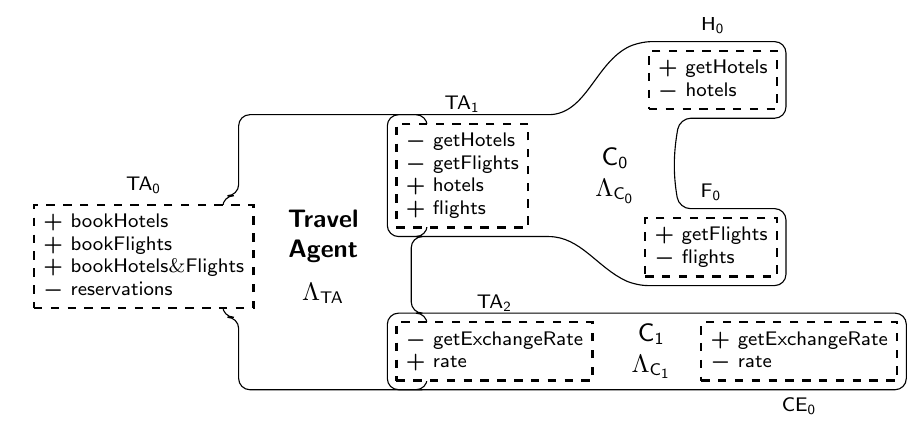
\includegraphics[scale=0.5]{images/ARN0.png}
\end{center}
Deseamos reemplazar los autómatas de Muller/finitos utilizados para describir procesos por algún tipo de autómata que pueda relacionar los aspectos computacionales del proceso con los comunicacionales declarados en sus puertos. Adicionalmente pretendemos un mecanismo de composición parcial, es decir que no requiera de todos los participantes al momento de realizar el binding.
\end{frame}

\begin{frame}{Autómatas Finitos de Comunicación Asincrónica}
\begin{itemize}
    \item Los Autómatas Finitos de Comunicación Asincrónica (AFCA) son una clase de autómatas de comunicación que poseen:
    \begin{itemize}
        \item Transiciones internas o de cómputo,
        \item Comunicación externa a través de los canales en $\mathcal{C}$
        \item Comunicación interna a través de buffers
    \end{itemize} 
    \item Permiten composición total y composición parcial internalizando la comunicación externa compartida entre participantes
    \item La interfaz de comunicación externa de un AFCA se puede proyectar en una communicating machine.(bajo ciertas condiciones que luego exploraremos)
\end{itemize}
\end{frame}

\begin{frame}{AFCA}
\begin{center}
\begin{tikzpicture}[->, thick, scale=0.5, every node/.style={transform shape}]
 \node[state,initial] (q_0)   {$q_0$}; 
 \node[state] (q_1) [right= 1.5cm of q_0 ] {$q_1$};
 \node[state] (q_2) [below= of q_0 ] {$q_2$};
 \node[state] (q_3) [right= 1.5cm of q_2 ] {$q_3$};
 \node[state, accepting] (q_4) [below= of q_3 ] {$q_4$};
	
 \draw[]        
        (q_0) edge[above] node{out(PR,a)} (q_1)
        (q_0) edge[left] node{in(SP,b)} (q_2)
        (q_1) edge[right] node{in(SP,b)} (q_3)
        (q_2) edge[above] node{out(PR,a)} (q_3)
        (q_3) edge[right] node{$int_p$} (q_4)
        ; 
\end{tikzpicture} 
\ 
\begin{tikzpicture}[->, thick,scale=0.5, every node/.style={transform shape}]
 \node[state,initial] (q_0)   {$q_0$}; 
 \node[state] (q_1) [below= of q_0 ] {$q_1$};
 \node[state, accepting] (q_2) [below= of q_1 ] {$q_2$};
 \draw[]        
        
        (q_0) edge[right] node{$int_r$} (q_1)
        (q_1) edge[right] node{in(pr,a)} (q_2)
        ;
\end{tikzpicture} 
\ 
\begin{tikzpicture}[->, thick,scale=0.5, every node/.style={transform shape}]
 \node[state,initial] (q_0)   {$q_0$}; 
 \node[state, accepting] (q_1) [below= of q_0 ] {$q_1$};

 \draw[]        
        
        (q_0) edge[right] node{out(sp,b)} (q_1)
        
        ;
\end{tikzpicture} 
\end{center}

\begin{center}
\begin{tikzpicture}[->, thick, scale=0.5, every node/.style={transform shape}]
 \node[state,initial] (q_0)   {$[q_0]$}; 
 \node[state] (q_1) [right= of q_0 ] {$[q_1]$};
  \node[state] (q_2) [below= of q_0 ] {$[q_2$]};
 \node[state] (q_3) [right= of q_2 ] {$[q_3]$};

 \draw[]        
        (q_0) edge[above] node{pr!a} (q_1)
        (q_0) edge[right] node{sp?b} (q_2)
        (q_1) edge[right] node{sp?b} (q_3)
        (q_2) edge[above] node{pr!a} (q_3)
        ; 
\end{tikzpicture} 
\
\begin{tikzpicture}[->, thick, scale=0.5, every node/.style={transform shape}]
 \node[state,initial] (q_0)   {$[q_0]$}; 
 \node[state] (q_1) [below= of q_0 ] {$[q_2]$};

 \draw[]        
        (q_0) edge[right] node{pr?a} (q_1)
        ;
\end{tikzpicture} 
\ 
\begin{tikzpicture}[->, thick, scale=0.5, every node/.style={transform shape}]
 \node[state,initial] (q_0)   {$[q_0]$}; 
 \node[state] (q_1) [below= of q_0 ] {$[q_1]$};
 
 \draw[]        
        (q_0) edge[right] node{sp!b} (q_1)
        ;
\end{tikzpicture} 
\end{center}
% \caption{mCFSM $M_P$, $M_R$ y $M_S$, correspondientes a los AFCAs de la Subfig.~\ref{a_i}.}
% \label{m_i}

Los AFCA P,R y S, y sus interfaces de comunicación.
\end{frame}

\begin{frame}{Composición parcial}
\begin{center}
\begin{tikzpicture}[->, thick, scale=0.6, every node/.style={transform shape}]
 \node[state,initial] (q_0)   {$q_0$}; 
 \node[state] (q_1) [right= 1.5cm of q_0 ] {$q_1$};
 \node[state] (q_2) [below= of q_0 ] {$q_2$};
 \node[state] (q_3) [right= 1.5cm of q_2 ] {$q_3$};
 \node[state, accepting] (q_4) [below= of q_3 ] {$q_4$};
	
 \draw[]        
        (q_0) edge[above] node{out(PR,a)} (q_1)
        (q_0) edge[left] node{in(SP,b)} (q_2)
        (q_1) edge[right] node{in(SP,b)} (q_3)
        (q_2) edge[above] node{out(PR,a)} (q_3)
        (q_3) edge[right] node{$int_p$} (q_4)
        ; 
\end{tikzpicture} 
\ 
\begin{tikzpicture}[->, thick,scale=0.6, every node/.style={transform shape}]
 \node[state,initial] (q_0)   {$q_0$}; 
 \node[state] (q_1) [below= of q_0 ] {$q_1$};
  \node[state] (q_2) [below= of q_1 ] {$q_2$};
  \node[state, accepting] (q_3) [below= of q_2 ] {$q_3$};
 \draw[]        
        
        (q_0) edge[right] node{$int_r$} (q_1)
        (q_1) edge[right] node{in(pr,a)} (q_2)
        (q_2) edge[right] node{out(rs,c)} (q_3)
        ;
\end{tikzpicture} 
\ 
\begin{tikzpicture}[->, thick,scale=0.6, every node/.style={transform shape}]
 \node[state,initial] (q_0)   {$q_0$}; 
 \node[state] (q_1) [below= of q_0 ] {$q_1$};
 \node[state, accepting] (q_2) [below= of q_1 ] {$q_2$};

 \draw[]        
        
        (q_0) edge[right] node{out(sp,b)} (q_1)
        (q_1) edge[right] node{in(rs,c)} (q_2)
        
        ;
\end{tikzpicture} 
\end{center}
    
\end{frame}


\begin{frame}{Composición parcial ejemplo}
\begin{tikzpicture}[->, thick,scale=0.5, every node/.style={transform shape}]
 \node[state,initial] (q_0)  {$q_{00}$}; 
 \node[state] (q_1) [ right=  3 of q_0] {$q_{01}$};
 \node[state] (q_2) [below = 1.5 of q_1 ] {$q_{11}$};
 \node[state] (q_3) [below = 2.5 of q_2 ] {$q_{12}$};
 \node[state] (q_4) [below left= and 3 of q_0] {$q_{10}$};
  \node[state] (q_6) [below = 1.5cm of q_4] {$q_{30}$};
  \node[state] (q_8) [below = and 3 of q_0 ] {$q_{20}$};
  \node[state] (q_9) [below =2 of q_8 ] {$q_{21}$};
  \node[state] (q_7) [below = of q_9] {$q_{31}$};
  \node[state] (q_5) [below right = of q_7 ] {$q_{32}$};
  \node[state] (q_10) [below left= of q_7] {$q_{41}$};
 \node[state] (q_11) [below= 3cm of q_7] {$q_{42}$};
 \node[state] (q_13) [below= of q_6] {$q_{40}$};
%  \node[state] (q_14) [below right= of q_5] {$q_{33}$}
 \node[state,accepting] (q_12) [below= of q_11] {$q_{43}$};
 \draw[]        
        (q_0) edge[above] node{$int_r$} (q_1)
        (q_0) edge[right] node{$in(SP,b)$} (q_8)
        (q_0) edge[below] node{$PR \ll a$} (q_4)
        (q_1) edge[right] node{$PR \ll a$} (q_2)
 		(q_2) edge[right] node{$PR \gg a$} (q_3)
    	(q_2) edge[right] node{$in(SP,b)$} (q_7)
        (q_3) edge[right] node{$in(SP,b)$} (q_5) 
        (q_4) edge[left] node{$in(SP,b)$} (q_6)
        (q_6) edge[left] node{$int_r$} (q_7)
        (q_6) edge[left] node{$int_p$} (q_13)
        (q_7) edge[right] node{$PR \gg a$} (q_5)
        (q_7) edge[left] node{$int_p$} (q_10)
        (q_10) edge[left] node{$PR \gg a$} (q_11)
        (q_8) edge[right] node{$int_r$} (q_9)
        (q_8) edge[above] node{$PR \ll a$} (q_6)
        (q_9) edge[right] node{$PR \ll a$} (q_7)
        (q_5) edge[right] node{$int_p$} (q_11)
        %  (q_5) edge[right] node{$Out(RS,C)$} (q_14)
        (q_11) edge[right] node{$Out(RS,C$} (q_12)
        (q_13) edge[left] node{$int_r$} (q_10)
        % (q_14) edge[right] node{$int_p$} (q_12)
        ;
\end{tikzpicture}
 \
\begin{tikzpicture}[->, thick,scale=0.6, every node/.style={transform shape}]
 \node[state,initial] (q_0)   {$q_0$}; 
 \node[state] (q_1) [below= of q_0 ] {$q_1$};
 \node[state, accepting] (q_2) [below= of q_1 ] {$q_2$};

 \draw[]        
        
        (q_0) edge[right] node{out(sp,b)} (q_1)
        (q_1) edge[right] node{in(rs,c)} (q_2)
        
        ;
\end{tikzpicture}

\end{frame}


\begin{frame}{MultiChannel CFSM y GMC}
\begin{itemize}
    \item \textbf{Multichannel Communicating Finite State Machines (mCFSM):} Son una extensión CFSMs con múltiples canales (al menos dos, uno en cada sentido) entre cada par de participantes.
    
    \item \textbf{Interfaz de comunicación de AFCA:} mediante un procedimiento extraemos el comportamiento comunicacional en la forma de una mCFSM
    
    \item \textbf{Sistema emulado:} Dado un multichannel CS $(M_p)_{p \in \mathcal{P}}$, agrandamos el conjunto $ \mathcal{P}$ agregando un participante adicional por cada canal en el sistema original $\mathcal{P}'=\mathcal{P} \cup \bigcup_{p \in \mathcal{P}} \{p^{pq_n} \ | \ pq_n \in \mathcal{C}_p \} \cup \bigcup_{p \in \mathcal{P}} \{p^{qp_n} \ | \ qp_n \in \mathcal{C}_p \}$. De este modo obtenemos un conjunto de CFSMs
    
    \item \textbf{GMC:} Como el sistema emulado preserva errores comunicacionales, podemos utilizar el criterio de GMC para el chequeo de compliance entre componentes
\end{itemize}

\end{frame}

\begin{frame}{Problema de las interfaces}

El primer problema es que no siempre ocurre. Como en este caso.

\begin{center}
\begin{tikzpicture}[->, thick,scale=0.6, every node/.style={transform shape}]
 \node[state,initial] (q_0)   {$q_0$}; 
 \node[state] (q_1) [below = of q_0 ] {$q_1$};
 \node[state] (q_2) [right = of q_1 ] {$q_2$};
 \node[state] (q_3) [below = of q_1 ] {$q_3$};
 \node[state] (q_4) [below = of q_2 ] {$q_4$};
 \draw[]        
        (q_0) edge[left] node{int1} (q_1)
        (q_0) edge[right] node{int2} (q_2)
        (q_1) edge[left] node{in(sp,a)} (q_3)
        (q_2) edge[right] node{in(sp,b)} (q_4)
        ; 
\end{tikzpicture}
\
\begin{tikzpicture}[->, thick,scale=0.6, every node/.style={transform shape}]
 \node[state,initial] (q_0)   {$q_0$}; 
 \node[state] (q_1) [below = of q_0 ] {$q_1$};
  \node[state] (q_2) [right = of q_1] {$q_2$};
 \draw[]        
        (q_0) edge[left] node{out(sp,a)} (q_1)
        (q_0) edge[right] node{out(sp,b)} (q_2)
        ; 
\end{tikzpicture}
\end{center}

\begin{center}

\begin{tikzpicture}[->, thick,scale=0.6, every node/.style={transform shape}]
 \node[state,initial] (q_0)   {$[q_0]$}; 
  \node[state] (q_1) [below = of q_0 ] {$[q_1]$};
 \node[state] (q_2) [right = of q_1 ] {$[q_2]$};
 \draw[]        
        (q_0) edge[left] node{sp?a} (q_1)
        (q_0) edge[right] node{sp?b} (q_2)
        ; 
\end{tikzpicture}
\
\begin{tikzpicture}[->, thick,scale=0.6, every node/.style={transform shape}]
 \node[state,initial] (q_0)   {$[q_0]$}; 
 \node[state] (q_1) [below = of q_0 ] {$[q_1]$};
  \node[state] (q_2) [right = of q_1 ] {$[q_2]$};
 \draw[]        
        (q_0) edge[left] node{sp!a} (q_1)
        (q_0) edge[right] node{sp!b} (q_2)
        ; 
\end{tikzpicture}
\end{center}
\end{frame}

\begin{frame}{Problema de las interfaces: Weak determinacy}
\begin{itemize}
    \item La proyección de comunicación no refleja el comportamiento real de los autómatas que en el ejemplo quedan en deadlock.
    \item No se puede tener una situación donde la decisión interna de un autómata afecte a los mensajes que este puede recibir.
    \item Hay una hipótesis en cada punto en donde nosotros proyectamos la interfaz de comunicación del autómata exigiendo que sea weak determinate.
    \item Weak determinacy garantiza que se pueden "ocultar" determinadas etiquetas sin afectar el comportamiento genral del autómata. En nuestro caso las de cómputo con las de comunicación.
\end{itemize}
\end{frame}

\begin{frame}{Equivalencia comunicacional}
Si chequeamos compliance entre un conjunto de interfaces, queremos que la composición de los AFCA originales al internalizar la comunicación, los elementos comunicacionales que ahora son parte del autómata compuesto preserva las propiedades del CS que usé para chequear compliance.
$$
\xymatrix{   
	\{\mathcal{A}_i\}_{i \in I} \ar[rrr]_{\Pi} \ar[d]_{||} & & & \{C_i\}_{i \in I}  \ar[d]_{semantica}  \\
	  {||_{i \in I}\{\mathcal{A}_i\}= \mathcal{A}} \ar[r]_{\ \ \ \ \Pi'} \ar[d]_{\Pi} & \mathcal{L}' & = & {\mathcal{L}}  \\
	  \emptyset
}
$$
\end{frame}

\begin{frame}{Proyección de comunicación interna}
\begin{itemize}
    \item Como precondición pedimos que el AFCA sea weak determinate y no tenga transiciones de comunicación externa
    \item Decimos que dos estados $q, q' \in Q$ son equivalentes por transiciones internas si puedo alcanzar $q'$ desde $q$ \textbf{sólo} por transiciones internas.
    \item Llamamos $[q]_m$ a la clase de equivalencia por transiciones internas de $q$, es decir todos los estados a los que puedo llegar \textbf{sólo} por transiciones internas 
    \item Tomamos las clases de equivalencia del AFCA
    \item Construimos el LTS con las tuplas $\langle [q]_m, \overrightarrow{\Omega} \rangle$, donde $\overrightarrow{\Omega}$ es el contenido de los buffers para ese estado
    \item Cada estado es una tupla que corresponde una configuración del autómata original desde la óptica de la comunicación
    \item Cada transición está etiquetada con la transición del autómata original que lleva de una configuración a la otra
\end{itemize}
\end{frame}

\begin{frame}{Proyección de comunicación interna}
Tomemos el siguiente AFCA
\begin{center}
\begin{tikzpicture}[->, thick, scale=0.6, every node/.style={transform shape}]
 \node[state,initial] (q_0)   {$q_{000}$}; 
 \node[state] (q_1) [right= 1.5cm of q_0 ] {$q_{100}$};
 \node[state] (q_2) [right = 1.5 of q_1 ] {$q_{110}$};
 \node[state] (q_12) [above right= 2 of q_2 ] {$q_{111}$};
  \node[state] (q_3) [below right= 2 of q_2 ] {$q_{120}$};
  \node[state] (q_4) [right = 3.1 of q_2 ] {$q_{121}$};
  \node[state] (q_5) [below= 4 of q_0] {$q_{001}$};
  \node[state] (q_6) [right = 1.5cm of q_5] {$q_{201}$};
   \node[state] (q_7) [above right = 2 of q_6 ] {$q_{301}$};
  \node[state] (q_11) [below = 3.5 of q_7] {$q_{211}$};
  \node[state] (q_8) [right = 3.5 of q_6] {$q_{311}$};
  \node[state] (q_9) [above right = 2 of q_8 ] {$q_{321}$};
  \node[state] (q_13) [below right= 2 of q_8 ] {$q_{411}$};
 \node[state,accepting] (q_10) [right= 3.5cm of q_8 ] {$q_{421}$};
 \draw[]        
        (q_0) edge[above] node{$PR \ll a$} (q_1)
        (q_1) edge[above] node{$int_r$} (q_2)
		(q_2) edge[left] node{$PR \gg a$} (q_3)
		(q_2) edge[left] node{$SP \ll b$} (q_12)
		(q_12) edge[left] node{$PR \gg a$} (q_4)
        (q_3) edge[left] node{$SP \ll b$} (q_4) 
        (q_4) edge[right] node{$SP \gg b$} (q_9)
        (q_0) edge[left] node{$SP \ll b$} (q_5)
        (q_5) edge[below] node{$SP \gg b$} (q_6)
        (q_6) edge[left] node{$PR \ll a$} (q_7)
        (q_6) edge[below] node{$int_r$} (q_11)
        (q_11) edge[right] node{$PR \ll a$} (q_8)
        (q_7) edge[right] node{$int_r$} (q_8)
        (q_8) edge[right] node{$int_p$} (q_13)
        (q_8) edge[right] node{$PR \gg a$} (q_9)
        (q_13) edge[right] node{$PR \gg a$} (q_10)
        (q_9) edge[above] node{$int_p$} (q_10)
        ;
\end{tikzpicture}
\end{center}
\end{frame}

\begin{frame}{Proyeción de comunicación interna}

\begin{center}
\begin{tikzpicture}[->, thick, scale=0.6, every node/.style={transform shape}]
    \node[state,initial] (q_0) {$[q_{000}],\epsilon, \epsilon$}; 
     \node[state] (q_1) [right= 3.5cm of q_0 ] {$[q_{100}], a, \epsilon$};
     \node[state] (q_2) [right = 3.5cm of q_1 ] {$[q_{120}],\epsilon,\epsilon$};
     \node[state] (q_8) [below= of q_1 ] {$[q_{111}], a, b$};
     \node[state] (q_3) [below= of q_2 ] {$[q_{121}],\epsilon, b$};
     \node[state] (q_4) [below=  of q_0] {$[q_{001}],\epsilon, b$};
     \node[state] (q_5) [below = of q_4] {$[q_{201}],\epsilon, \epsilon$};
     \node[state] (q_6) [right = 3.5cm of q_5 ] {$[q_{301}], a, \epsilon$};
     \node[state,accepting] (q_7) [below = of q_3 ] {$[q_{321}],\epsilon, \epsilon$};
\draw[]        
     (q_0) edge[above] node{$\langle q_{000}, PR \ll a, q_{100} \rangle$} (q_1)
	 (q_1) edge[above] node{$\langle q_{110}, PR \gg a, q_{120} \rangle$} (q_2)
	 (q_1) edge[left] node{$\langle q_{110}, SP \ll b, q_{111} \rangle$} (q_8)
	 (q_8) edge[above] node{$\langle q_{111}, PR \gg a, q_{121} \rangle$} (q_3)
     (q_2) edge[left] node{$\langle q_{120}, SP \ll b, q_{121} \rangle$} (q_3) 
     (q_3) edge[left] node{$\langle q_{121}, SP \gg b, q_{321} \rangle$} (q_7)
     (q_0) edge[left] node{$\langle q_{000}, SP \ll b, q_{001} \rangle$} (q_4)
     (q_4) edge[left] node{$\langle q_{001}, SP \gg b, q_{201} \rangle$} (q_5)
     (q_5) edge[below] node{$\langle q_{201}, SP \gg b, q_{301} \rangle$} (q_6)
     (q_6) edge[below] node{$\langle q_{311}, PR \ll a, q_{321} \rangle$} (q_7)
      ;
\end{tikzpicture}
\end{center}
\end{frame}

\begin{frame}{Equivalencia Comunicacional}
Para ver que la composición preserva la semántica comunicacional de un conjunto de AFCA  y sus respectivas mCFSMs queremos probar que $\widehat{\mathcal{A}}$ y $M$ son bisimilares. Para lo cual necesitamos que: 
\begin{enumerate}
    \item $\{\mathcal{A}\}_{1 \leq i \leq n}$ sea un conjunto de weak determinate AFCA sin transiciones de comunicación interna
    \item su composición $\mathcal{A}$, también es weak determinate
    \item $\widehat{\mathcal{A}}$ el sistema de transición etiquetado (LTS) que resulta de la proyección $\Tau(\mathcal{A})$
    \item $\{M_i\}_{1 \leq i \leq n}$ de mCFSM correspondientes a cada uno de los AFCAs
    \item $M = \langle P, \mathcal{C}, {p_0}, [\delta] \rangle$ el LTS que representa la semántica del CS
\end{enumerate}
\end{frame}

\begin{frame}{Equivalencia Comunicacional}
Dadas las condiciones establecidas necesitamos probar:
\begin{enumerate}
    \item \textbf{Equivalencia de estados discretos:} Para todo $\langle [\overrightarrow{q}]_m, \overrightarrow{\Omega} \rangle \in \widehat{Q}$, existe $\langle \overrightarrow{p}, \overrightarrow{\Omega_{\mathcal{C}}} \rangle \in P$ tal que $q_i \in \overrightarrow{q} \iff q_i \in \overrightarrow{p}$ y viceversa.
    \item \textbf{Equivalencia entre buffers y canales:} Dados $\langle [\overrightarrow{q}]_m, \overrightarrow{\Omega} \rangle \in \widehat{Q}$ y $\langle \overrightarrow{p}, \overrightarrow{\Omega_{\mathcal{C}}} \rangle \in P$. Queremos ver que el conjunto de buffers $B$ de $\mathcal{A}$ es el conjunto de canales internalizados de $\mathcal{C}$ de $M$. Es decir que para todo canal $\omega$ vale que $\omega \in \mathcal{C}$ si y solo si $\omega \in B$
    \item \textbf{Equivalencia de las semánticas de las mFCSMs y los AFCAs:} Queremos ver que para todo para todo par de estados bisimilares $\widehat{q}=\langle [\overrightarrow{q}]_m, \overrightarrow{\Omega} \rangle \in \widehat{Q}$ y $p=\langle [\overrightarrow{q}]_m, \overrightarrow{\Omega} \rangle \in \widehat{Q}$, queremos probar que para toda transición que vaya de $\widehat{q}$ a $\widehat{q'}$ existe $p' \in P$, alcanzable desde $p$, tal que $\widehat{q'}$ y $p'$ son bisimilares. Y simétricamente para toda transición que vaya de $p$ a $p'$, existe $\widehat{q'} \in \widehat{Q}$, alcanzable desde $\widehat{q}$, tal que $\widehat{q'}$ y $p'$ son bisimilares
\end{enumerate}
    
\end{frame}

\begin{frame}{Conclusiones}
El objetivo de esta tesis era el estudio y posible extensión de los modelos formales para servicios, partiendo del ideal de SOC un contexto que permita la reconfiguración dinámica de un artefacto de software a partir de posibilitar el binding en tiempo de ejecución. Para esto desarrollamos:
\begin{itemize}
    \item Un formalismo que soporte binding parcial, los AFCA que permiten internalizar el intercambio de mensajes como comportamiento interno al componer, preservando la comunicación externa de las componentes.
    \item Para expresar la interfaz externa de comunicación de los AFCA propusimos las mCFSMs
    \item Como método para garantizar que los distintos participantes puedan interoperar en forma segura extendimos la noción de GMC para mCFSM
    \item Por último pudimos demostrar la equivalencia entre el comportamiento de la composición de un conjunto de AFCA y el de sus respectivas mCFSMs
\end{itemize}
\end{frame}

\begin{frame}{Trabajo futuro}
\begin{itemize}
    \item Queda por estudiar en mayor profundidad si el lenguaje cumple con las condiciones esperadas.
    \item Definir formalmente la composición parcial de AFCAs y ver la relación entre un AFCA obtenido por una serie de composiciones parciales y uno de una composición total
    \item Ver si es posible lingüísticamente generar autómatas weak determinate que al componerse den uno que también lo sea
    \item Autómatas con comportamiento interno encapsulado los estados?
\end{itemize}

    
\end{frame}

\bibliographystyle{alpha}
\bibliography{bibdatabase}
\end{document}
